\documentclass{beamer}
%
% Choose how your presentation looks.
%
% For more themes, color themes and font themes, see:
% http://deic.uab.es/~iblanes/beamer_gallery/index_by_theme.html
%
\mode<presentation>
{
  \usetheme{Boadilla}      % or try Darmstadt, Madrid, Warsaw, ...
  \usecolortheme{seahorse} % or try albatross, beaver, crane, ...
  \usefonttheme{default}  % or try serif, structurebold, ...
  \setbeamertemplate{navigation symbols}{}
  \setbeamertemplate{caption}[numbered]
  \setbeamertemplate{bibliography item}{\insertbiblabel}
}

\usepackage[english]{babel}
\usepackage[utf8]{inputenc}
\usepackage{xcolor}
\usepackage[T1]{fontenc}
\usepackage{graphicx}
\usepackage[style=numeric,backend=biber]{biblatex}
\setbeamerfont{footnote}{size=\tiny}
\usepackage{caption}
\usepackage{subcaption}
\usepackage{amsmath}

\addbibresource{bibliography.bib}
\title[Distributed Delays in R-D systems]{Distributed Delays in Reaction-Diffusion Systems}

\author[A Sargood, A Krause, E Gaffney ]{Alec Sargood\\Supervisors: Andrew Krause and Eamonn Gaffney}

\begin{document}

\begin{frame}
  \titlepage
\end{frame}

\begin{frame}{What is a Turing pattern ? \cite{murray}}
    \begin{itemize}
    \item Turing proposed chemical basis for biological pattern formation (Reaction-Diffusion systems) \cite{turing}.
    \item Turing (diffusion-driven) instability: spatially homogeneous steady state $+diffusion\implies$ spatially inhomogenous steady-state.
    \begin{equation}
        u_t=\nabla^2u+f(u,v),\quad \quad v_t=d\nabla^2v+g(u,v)
    \end{equation}
    \item Linearising about steady-state (no diffusion):
    \begin{itemize}
        \item $f_u+g_v<0, \quad \quad f_ug_v-f_vg_u>0$
    \end{itemize}
    \item Linearising about steady-state (with diffusion):
    \begin{itemize}
        \item $df_u+g_v>0, \quad \quad (df_u+g_v)^2-4d(f_ug_v-f_vg_u)>0$
    \end{itemize}
\end{itemize}
\end{frame}

\begin{frame}{Turing patterns in nature}
    \begin{figure}[H]
        \begin{subfigure}[b]{0.45\linewidth}
            \centering
            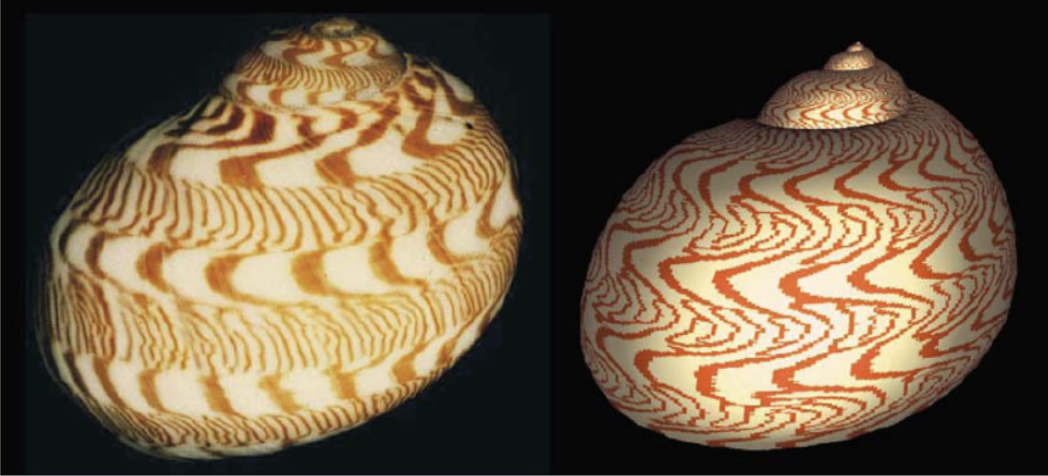
\includegraphics[width=5.5cm,height=4cm]{shell.png}
            \caption{Image taken from \cite{turing1}}
        \end{subfigure}
        \begin{subfigure}[b]{0.45\linewidth}
            \centering
            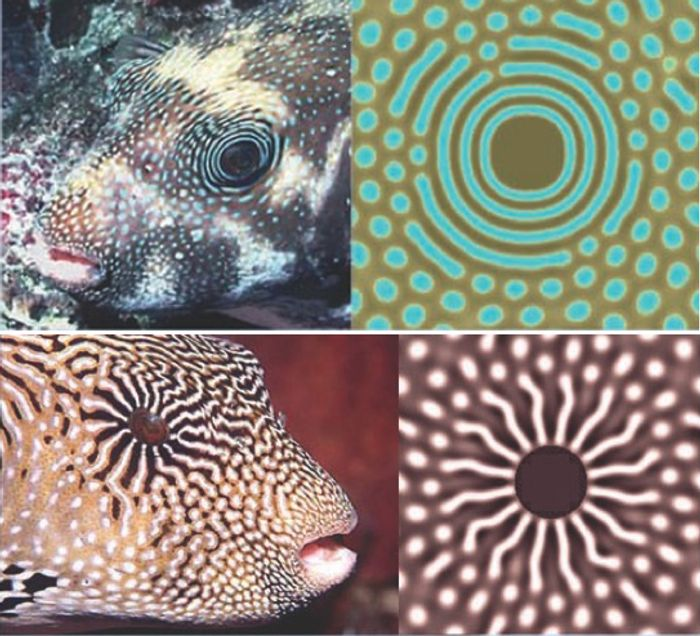
\includegraphics[width=5.5cm,height=4cm]{turing1.png}
            \caption{Image taken from \cite{nature}}
        \end{subfigure}
        \caption{Patterns found in nature}
    \end{figure}

\end{frame}
\begin{frame}{Mathematical Model (Without delay)}
        \begin{itemize}
            \item Schnakenberg Kinetics. $u=u(x,t), v=v(x,t)$.
        \end{itemize}
            \begin{equation}
                \begin{pmatrix}
                    u_t\\
                    v_t
                \end{pmatrix}
                =
                \begin{pmatrix}
                    u_{xx}\\
                    dv_{xx}
                \end{pmatrix}
                +
                \begin{pmatrix}
                    a-u+u^2v\\
                    b-u^2v
                \end{pmatrix}
            \end{equation}

            \begin{itemize}
                \item Conditions for Turing instability:
                \begin{itemize}
                    \item $0<b-a<(a+b)^3$
                    \item $(a+b)^2>0$
                    \item $d(b-a)>(a+b)^3$
                    \item $\left[d(b-a)-(a+b)^3\right]^2>4d(a+b)^4$
                \end{itemize}
            \end{itemize}
            \begin{figure}[H]
                \centering
                    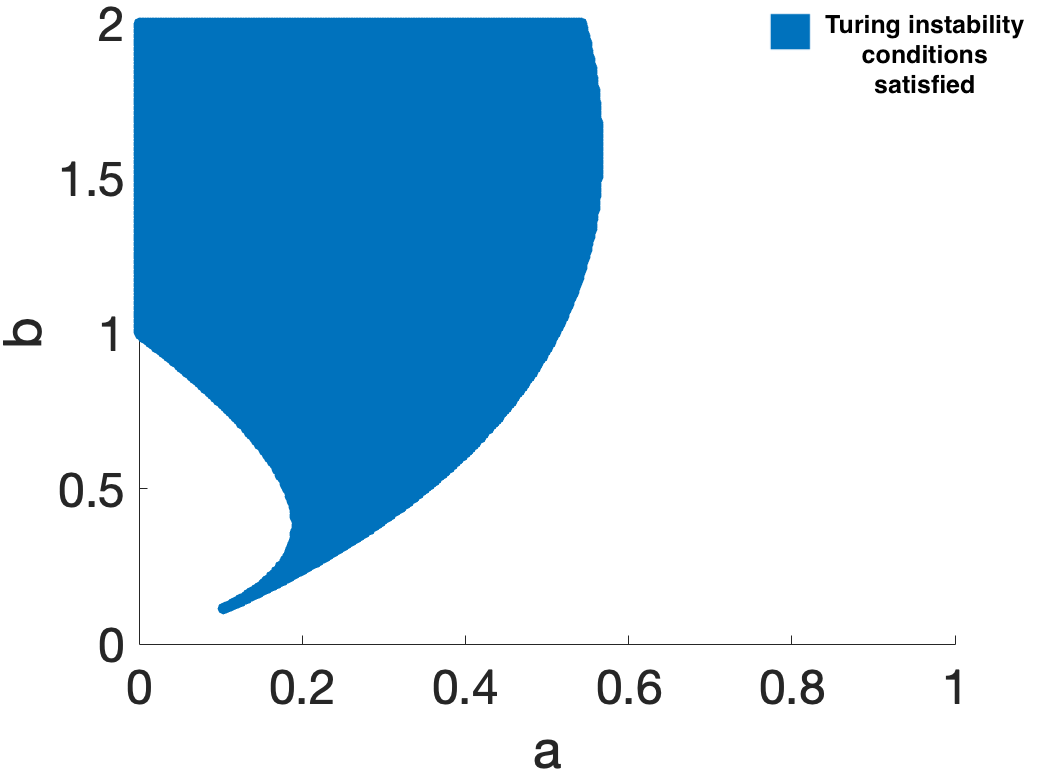
\includegraphics[width=5.5cm,height=3.2cm]{tspace.png}
                    \caption{Turing space produced in MATLAB}
            \end{figure}

\end{frame}

\begin{frame}{Research Aims}
\begin{itemize}
  \item Question: How does (distributed) delay affect the propensity for Turing instability and pattern formation ?

  \item Motivation:\begin{itemize}
  \item Time-delays affect behaviour of dynamical systems.
  \item Arise naturally in gene-expression process.
  \item Can affect the type and timing of pattern formation that we see.
\end{itemize}
\end{itemize}

\begin{figure}[H]
    \begin{subfigure}[b]{0.45\linewidth}
        \centering
        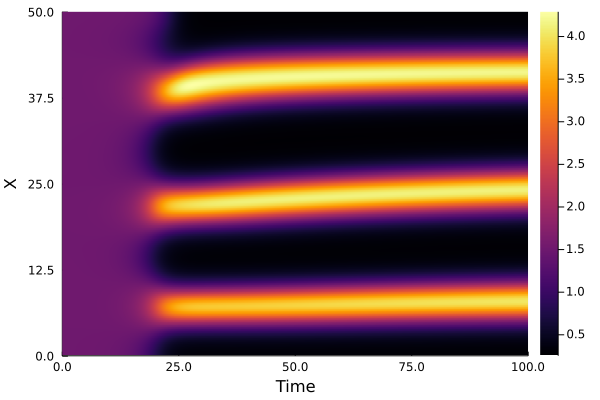
\includegraphics[width=5cm,height=4cm]{NoDelaySpatial.png}
        \caption{Example of Turing pattern produced in Julia (without delay)}
    \end{subfigure}
    \begin{subfigure}[b]{0.45\linewidth}
        \centering
        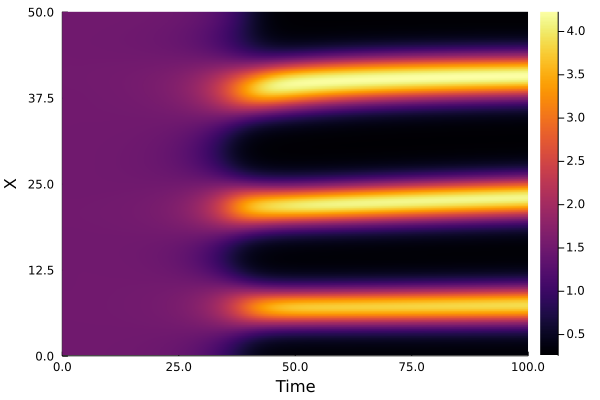
\includegraphics[width=5cm,height=4cm]{Fixedτ0.2.png}
        \caption{Example of Turing pattern produced in Julia (with delay)}
    \end{subfigure}
\end{figure}
\end{frame}

\begin{frame}{Biological Motivation \cite{gaffmonk,william}}
\begin{itemize}
    \item Ability of cell to adopt state relevant to its spatial and temporal position (Differential gene expression).
    \item Cell-signalling: co-ordination among cells.
    \item Cell-signalling influence the gene-expression process, ultimately resulting in spatial pattern formation.
    \item Gene expression is complex (gene-transcription, translation) with time-delays (in reality are stochastic.)
\end{itemize}

\begin{figure}[H]
        \centering
        \hspace*{6cm}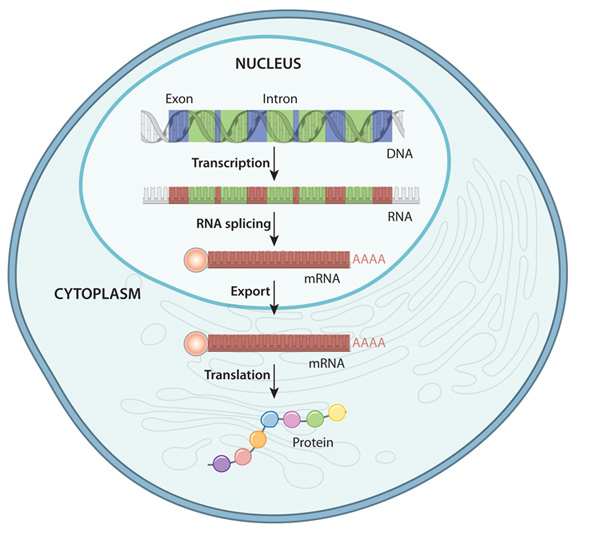
\includegraphics[width=5cm,height=3.8cm]{geneexp.png}
        \caption{An overview of the flow of information from DNA to protein in a cell \cite{nature}}
    \end{figure}
\end{frame}

\begin{frame}{Mathematical Model (With delay)}
    \begin{itemize}
        \item Ligand-Internalisation model. $u=u(x,t), v=v(x,t)$.
        \begin{itemize}

        \item With fixed time-delay
        \begin{equation}
            \begin{pmatrix}
                u_t\\
                v_t
            \end{pmatrix}
            =
            \begin{pmatrix}
                u_{xx}\\
                dv_{xx}
            \end{pmatrix}
            +
            \begin{pmatrix}
                a-u-2u^2v+3\textcolor{red}{u^2(t-\tau)v(t-\tau)}\\
                b-u^2v
            \end{pmatrix}
        \end{equation}


        \item With distributed time-delay

        \begin{equation}
            \begin{pmatrix}
                u_t\\
                v_t
            \end{pmatrix}
            =
            \begin{pmatrix}
                u_{xx}\\
                dv_{xx}
            \end{pmatrix}
            +
            \begin{pmatrix}
                a-u-2u^2v+3\textcolor{red}{\int_0^{2\tau}k(s,\tau,\sigma)u^2(t-s)v(t-s) ds}\\
                b-u^2v
            \end{pmatrix}
        \end{equation}

        $k(s,\tau,\sigma)$ truncated Gaussion pdf, mean: $\tau$, standard deviation: $\sigma$.

    \end{itemize}
\end{itemize}
We consider homogeneous Neumann boundary conditions (self-organisation), and restrict our investigation to one spatial dimension.
\end{frame}

\begin{frame}{Current Literature}

    \begin{itemize}
        \item Currently literature mostly describes the fixed delay case \cite{gaffmonk,paper1,paper2}. Fixed delays can:
        \begin{itemize}
            \item Increase time to pattern formation.
            \item Result in temporal oscillations (shrinking Turing space.)
            \item Increase sensitivity of patterns to initial conditions.
    \end{itemize}

\begin{figure}[H]
        \centering
        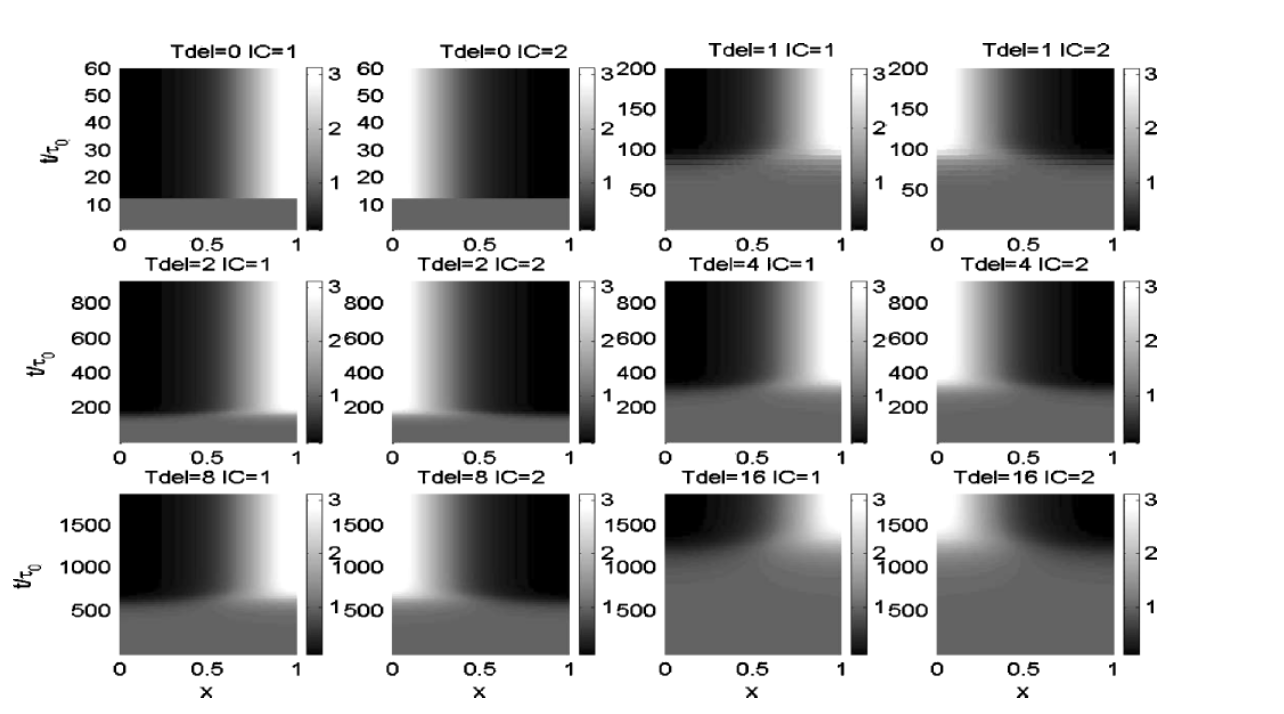
\includegraphics[width=11cm,height=4.5cm]{picDelay.png}
        \caption{Result of fixed time-delay \cite{gaffmonk}}
\end{figure}

\item Does distributed delay alleviate (or worsen) some of these problems ?
\end{itemize}

\end{frame}

\begin{frame}{Report Structure (1)}
    \begin{itemize}
        \item 1. Development and validation of tools
        \begin{itemize}
            \item Gauss-Hermite quadrature to approximate distributed delay as a set of $N$ fixed delay. Integrals of the form
            \begin{equation}
                \int_{-\infty}^{\infty}e^{-x^2}f(x)\approx\sum_{i=1}^Nw_if(x_i)
            \end{equation}
            \begin{itemize}
                \item Quadrature method builds off work in \cite{william}.
            \end{itemize}
            \item Use Julia to numerically solve stiff DDEs.
            \begin{itemize}
                \item Efficient code for our purposes.
            \end{itemize}
            \item Verify results against current literature/analytical examples/convergence analysis.
        \end{itemize}
    \end{itemize}

\end{frame}

\begin{frame}{Report Structure (2)}

    \begin{itemize}
        \item 2. Review of current literature and further analysis (Fixed delay)
        \begin{itemize}
            \item Validation of results.
            \item Sensitivity of results to initial conditions - systematic extension.
            \item How do varying model parameters affect these results.
            \begin{itemize}
                \item Higher risk: depends on computational limits
            \end{itemize}

        \end{itemize}
    \end{itemize}
    \begin{figure}[H]
        \begin{subfigure}[b]{0.45\linewidth}
            \centering
            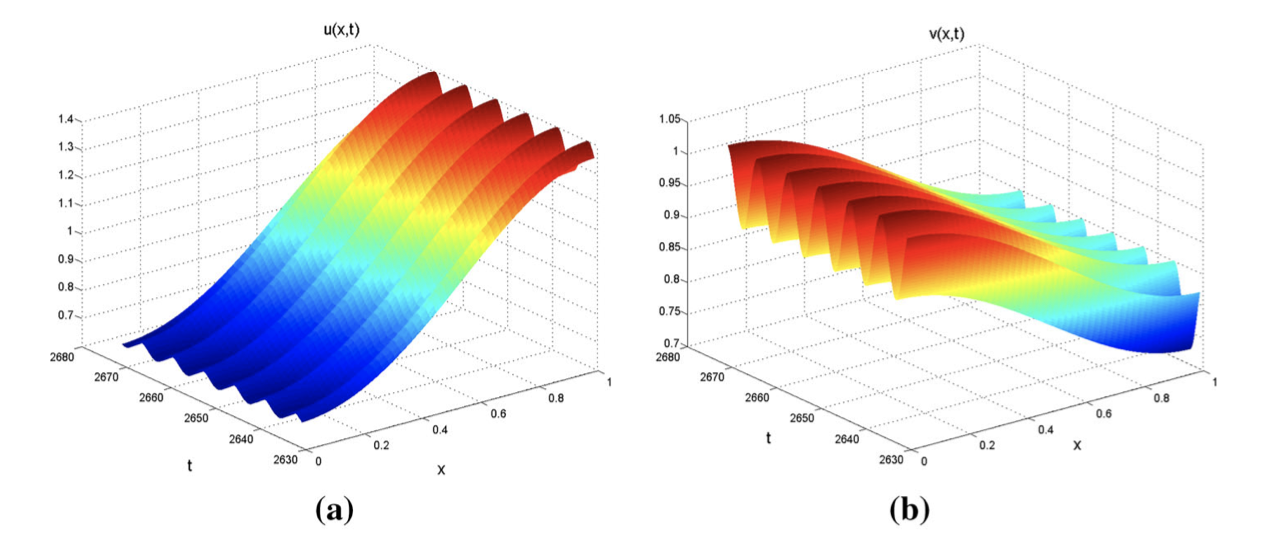
\includegraphics[width=6cm,height=3cm]{res1.png}
            \caption{Results produced in \cite{jiang}}
        \end{subfigure}
        \begin{subfigure}[b]{0.45\linewidth}
            \centering
            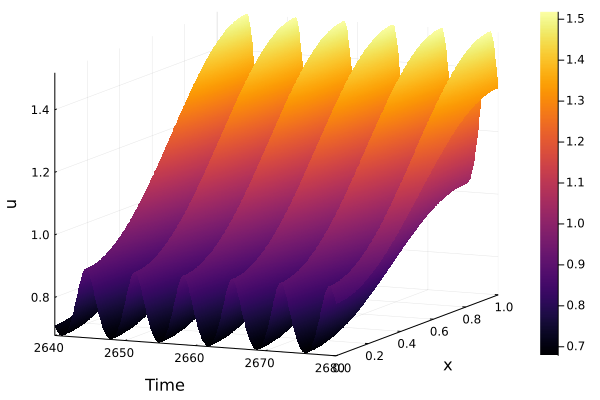
\includegraphics[width=6cm,height=3cm]{repres.png}
            \caption{Results reproduced in Julia}
        \end{subfigure}
    \end{figure}
\end{frame}

\begin{frame}{Report Structure (3)}
    \begin{itemize}
        \item 3. Incorporate distribution
        \begin{itemize}
            \item Analysis of varying $\sigma$
            \begin{itemize}
                \item No current literature on distributed delay in Schnakenberg model.
                \item Previous dissertation - preliminary results.
            \end{itemize}
            \item Consider different distributions/delay terms
            \begin{itemize}
                \item Higher risk: depends on research time limits
            \end{itemize}
        \end{itemize}
    \end{itemize}

    \begin{figure}[H]
        \begin{subfigure}[b]{0.32\linewidth}
            \centering
            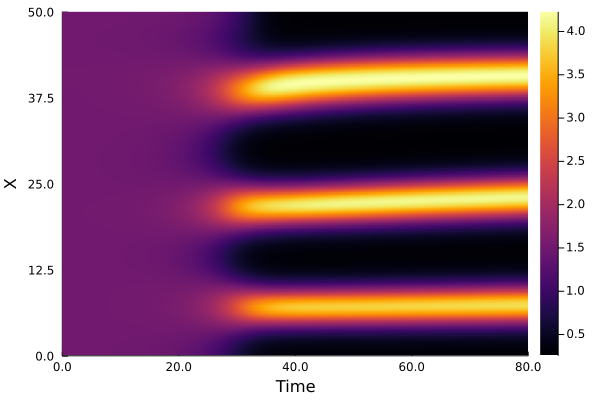
\includegraphics[width=4cm,height=3cm]{pic1.png}
            \caption{$\tau=0.4, \sigma=0.1$}
        \end{subfigure}
        \begin{subfigure}[b]{0.32\linewidth}
            \centering
            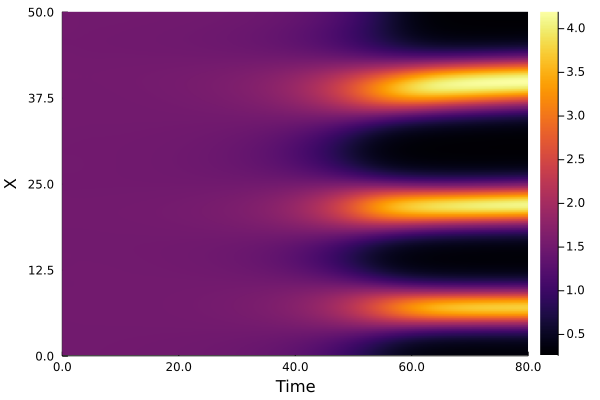
\includegraphics[width=4cm,height=3cm]{pic2.png}
            \caption{$\tau=0.6, \sigma=0.01$}
        \end{subfigure}
        \begin{subfigure}[b]{0.32\linewidth}
            \centering
            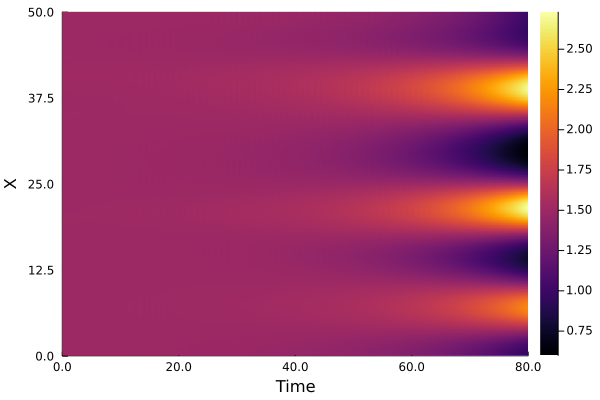
\includegraphics[width=4cm,height=3cm]{pic3.png}
            \caption{$\tau=0.8, \sigma=0.01$}
        \end{subfigure}
        \caption{Results produced in Julia}
    \end{figure}

\end{frame}


\begin{frame}{Report Structure (4)}
    \begin{itemize}
        \item 4. Summary and Conclusion
        \begin{itemize}
            \item Developed efficient code to numerically solve stiff DDEs.
            \hfill
            \item Evaluation of current literature for fixed delays and systematic extension.
            \hfill
            \item Understanding impact of distributed delays.
            \hfill
            \item Goal: Does the prospect of Turing patterns increase or decrease with distributed delays.

        \end{itemize}
    \end{itemize}
\end{frame}


\begin{frame}{References}
\AtNextBibliography{\tiny}
\printbibliography
\end{frame}
\end{document}
